\documentclass[12pt, letter]{exam}
\usepackage[utf8]{inputenc}
\usepackage[T1]{fontenc}
\usepackage[spanish]{babel}
\usepackage{amsmath}
\usepackage{amsthm}
\usepackage{physics}
\usepackage{tikz}
\usepackage{float}
\usepackage{siunitx}
\usepackage{multicol}
\usepackage[left=2.00cm, right=2.00cm, top=2.00cm, 
     bottom=2.00cm]{geometry}
\usepackage{pdfpages}
\usepackage{enumitem}
\usepackage{circuitikz}

% \renewcommand{\questionlabel}{\thequestion}
\decimalpoint

\setlength{\belowdisplayskip}{-0.5pt}

\usepackage{tasks}
\settasks{
    label=\Alph*), 
    label-align=left,
    item-indent={20pt}, 
    column-sep={4pt},
    label-width={16pt},
}

\sisetup{per-mode=symbol}
\footer{}{\thepage}{}

\begin{document}

\includepdf[pages=-]{Caratula_Examen_Parcial_04_PU_Fisica_4_01_Grupo_93.pdf}
\setcounter{page}{3}

\newpage
\begin{center}
\textbf{Cada ejercicio vale 1 punto, incluidos los de ejecución.}
\end{center}

\begin{questions}

    \section{(10 puntos) Instrumentación biomédica.}

    \question El estetoscopio Pinard es un tipo de instrumento de diagnóstico que se clasifica en el grupo de estetoscopios: \rule{2cm}{0.1mm}
    \begin{tasks}(4)
        \task Automático.
        \task Electrónico.
        \task Mecánico.
        \task Estándar.
    \end{tasks}
    \question El mm Hg representa una unidad derivada de presión equivalente \rule{2cm}{0.1mm} de una columna de mercurio de \rule{2cm}{0.1mm} de altura.
    \begin{tasks}(4)
        \task al peso - \SI{1}{\meter}
        \task a 1 Newton - \SI{1}{\meter}
        \task a la masa - \SI{1}{\milli\meter}
        \task al peso - \SI{1}{\milli\meter}
    \end{tasks}
    \question Con el esfigmomanómetro se registran dos valores de presión arterial, el primero y más alto corresponde a la presión: \rule{2cm}{0.1mm}
    \begin{tasks}(4)
        \task Intraarticular.
        \task Sistólica.
        \task Diastólica.
        \task Abdominal.
    \end{tasks}
    \question El inicio de los ruidos de Korotkoff se presenta cuando la presión \rule{2cm}{0.1mm} es \rule{2cm}{0.1mm} que la presión del brazalete del esfigmomanómetro.
    \begin{multicols}{2}
    \begin{tasks}
        \task Sistólica - Mayor
        \task Diastólica - Mayor
        \task Diastólica - Menor
        \task Sistólica - Menor
    \end{tasks}
    \end{multicols}
    \question Es el tipo de radiación ionizante que se utiliza en equipos de tomografía axial computarizada y que es absorbida por el tejido biológico: \rule{2cm}{0.1mm}
    \begin{multicols}{2}
    \begin{tasks}
        \task Rayos Ultravioleta.
        \task Rayos X.
        \task Rayos Infrarrojos.
        \task Rayos Gamma.
    \end{tasks}
    \end{multicols}
    \question Con un equipo de ultrasonido se envían ondas sonoras al cuerpo, el fenómeno que se presenta entre las ondas y el cuerpo es la \rule{2cm}{0.1mm}, que permite el registro y reconstrucción en una imagen bidimensional de la zona anatómica.
    \begin{tasks}(4)
        \task Refracción
        \task Rarefacción
        \task Reflexión
        \task Compresión
    \end{tasks}

    \newpage

    \question A continuación se presenta un conjunto de instrumentos biomédicos, relaciona si son invasivos (inv) o no invasivos (noinv)
    \begin{multicols}{2}
        I. Esfigmomanómetro \\
        II. Rayos X  \\
        III. Ultrasonido \\
        IV. Electrocardiograma \\
        V. Resonancia magnética nuclear \\
        VI. Tomografía axial computarizada \\
        VII. Estetoscopio \\
        VIII. Oxímetro
    \end{multicols}

    \vspace{0.3cm}
    Respuestas:
    \begin{tasks}
        \task noinv-I, inv-II, inv-IV, noinv-VI
        \task inv-II, inv-III, noinv-VI, noinv-VIII
        \task noinv-V, inv-VI, noinv-VII, noinv-VIII
        \task inv-II, noinv-III, noinv-VII, inv-VIII
    \end{tasks}
    \question En un electroencefalograma (EEG), son las ondas que indican un estado de alerta, consciencia y concentración: \rule{2cm}{0.1mm}
    \begin{tasks}(4)
        \task Alfa $(\alpha)$.
        \task Beta $(\beta)$.
        \task Gamma $(\gamma)$.
        \task Delta $(\delta)$.
    \end{tasks}
    \question La longitud de onda $(\lambda)$ de los Rayos X, es \rule{2cm}{0.1mm} en comparación con la longitud de onda de la región visible.
    \begin{tasks}(4)
        \task Mayor
        \task Menor
        \task El doble
        \task La mitad
    \end{tasks}
    \question Apellido del científico que desarrolló las bases del electrocardiograma (EKG):
    \begin{tasks}(4)
        \task Lippmnann
        \task Galvani
        \task Einthoven
        \task Berger
    \end{tasks}

    \section{(10 puntos) Potencial de acción.}

    \question Se llama \rule{2cm}{0.1mm} al ion que ha perdido electrones.
    \begin{tasks}(4)
        \task Catión
        \task Anión
        \task Neutro
        \task Monoatómico        
    \end{tasks}
    \question En el proceso de difusión, una sustancia tiende a moverse de una zona de \rule{2cm}{0.1mm} concentración a un área de \rule{2cm}{0.1mm} concentración hasta que esta sea igual a lo largo de un espacio.
    \begin{tasks}(4)
        \task Menor - Mayor
        \task Mayor - Menor
        \task Mayor - Igual
        \task Igual - Igual
    \end{tasks}
    \question Es un ion cuya concentración a nivel intracelular es mayor que a nivel extracelular, hablamos del: \rule{2cm}{0.1mm}
    \begin{tasks}(4)
        \task Sodio (Na+)
        \task Cloro (Cl-)
        \task Sulfuro (S2-)
        \task Potasio (K+)
    \end{tasks}
    \question Es el tipo de célula que responde ante la estimulación directa con una corriente eléctrica, hablamos de: \rule{2cm}{0.1mm}.
    \begin{tasks}(4)
        \task Neurona.
        \task Eritrocito.
        \task Melanocito.
        \task Adipocito.
    \end{tasks}
    \question Cuando hablamos de la diferencia en las concentraciones iónicas a nivel intra y extracelular, que condiciona una diferencia entre las cargas a ambos lados de la membrana, las mismas que tratarán de igualarse, hablamos del equilibrio de: \rule{2cm}{0.1mm}
    \begin{tasks}(4)
        \task Hodgkin
        \task Huxley
        \task Goldman-Katz
        \task Gibbs-Donnan
    \end{tasks}
    \question Una característica del potencial de acción: es un cambio \rule{2cm}{0.1mm} en el potencial de membrana que ocurren en células excitables.
    \begin{tasks}(4)
        \task Lineal.        
        \task Pausado.        
        \task Exponencial.        
        \task Súbito.        
    \end{tasks}
    \question Es el momento en el que se abren los canales de Na+ y al ingresar a la parte interna de la célula, se modifica el signo del potencial eléctrico: \rule{2cm}{0.1mm}
    \begin{tasks}(4)
        \task Repolarización.
        \task Despolarización.
        \task Per. Refractario.
        \task Sobretiro.
    \end{tasks}
    \question Los canales de \rule{2cm}{0.1mm} se abren para regresar al estado de reposo en el interior de la célula.
    \begin{tasks}(4)
        \task K+
        \task Cl-
        \task Ca2+
        \task NH4+
    \end{tasks}

    \newpage

    \question Se presenta a continuación una gráfica del potencial de acción, relaciona las fases (inciso con minúsculas) con un número romano en la gráfica.
    \begin{figure}[H]
        \centering
        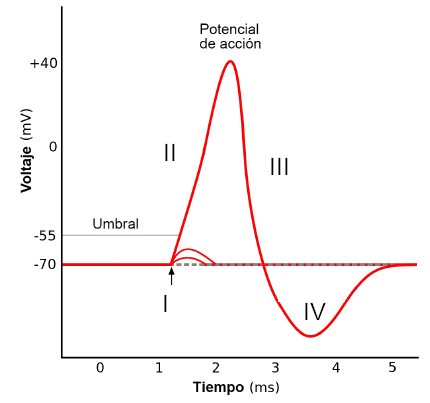
\includegraphics[scale=0.75]{Potencial_Accion_07.png}
    \end{figure}

    Fases del potencial de acción:
    \renewcommand{\thepartno}{\alph{partno}}
    \begin{multicols}{2}
    \begin{parts}
        \part Estímulo
        \part Reposo
        \part Repolarización
        \part Período refractario
        \part Despolarización
         \vspace*{\fill}
    \end{parts}
    \end{multicols}

    Opciones de respuesta:
    \begin{multicols}{2}
    \begin{tasks}
        \task I-a, II-d, III-b, IV-e
        \task I-e, II-b, III-d, IV-c
        \task I-a, II-e, III-c, IV-d
        \task I-a, II-e, III-c, IV-b
    \end{tasks}
    \end{multicols}
    \question En la hiperpolarización se requiere que el estímulo sea de \rule{2cm}{0.1mm} intensidad que el primer estímulo que provocó el primer potencial de acción.
    \begin{tasks}(4)
        \task Igual
        \task Mayor
        \task Menor
        \task Cero
    \end{tasks} 

\end{questions}

% \newpage

% \textbf{\huge{Formulario.}}
% \begin{table}[H]
%     \centering
%     \setlength{\tabcolsep}{40pt}
%     \renewcommand{\arraystretch}{2.5}
%     \begin{tabular}{c  c}
%         \multicolumn{2}{c}{Ondas} \\
%         $v = \lambda \, f$ & $T = \dfrac{1}{f}$ \\ \hline
%         \multicolumn{2}{c}{Sonido} \\
%         $B = 10 \, \log \left( \dfrac{I}{I_{0}} \right)$ & $I_{0} = \SI{1d-12}{\watt\per\square\meter}$ \\
%         $\lambda = \dfrac{2 \, L}{n}$ & $f^{\prime} = \dfrac{f \, V}{V \pm v}$ \\
%         $f^{\prime} = \dfrac{f \, (V \pm v)}{v}$ & \\ \hline
%         \multicolumn{2}{c}{Óptica geométrica} \\
%         $n = \dfrac{\text{sen} \, i}{\text{sen} \, i}$ & $n_{a} \, \text{sen} \,  a = n_{b} \, \text{sen} \,  b$ \\ \hline
%         \multicolumn{2}{c}{Lentes delgadas} \\
%         $\dfrac{1}{f} = \dfrac{1}{d_{o}} + \dfrac{1}{d_{i}}$ (lente convergente) & $- \dfrac{1}{f} = \dfrac{1}{d_{o}} - \dfrac{1}{d_{i}}$ (lente divergente) \\
%         $m = - \dfrac{d_{i}}{d_{o}} = \dfrac{h_{i}}{h_{o}}$ & $\text{Potencia } = \dfrac{1}{f} \quad f \text{ en } \unit{\meter}$ \\ \hline
%         \multicolumn{2}{c}{Hidrodinámica} \\
%         $G = \dfrac{V}{t}$ & $G = A \, v$ \\
%         $\text{Flujo} = \dfrac{m}{t}$ & $\text{Flujo} = \dfrac{\rho \, V}{t}$ \\
%         $\text{Flujo} = G \, \rho$ & \\
%         $v_{1} \, A_{1} = v_{2} \, A_{2}$ & $v = \sqrt{2 \, g \, h}$ \\
%         \multicolumn{2}{c}{$P_{1} + \rho \, g \, h_{1} + \dfrac{1}{2} \rho \, v_{1}^{2} = P_{2} + \rho \, g \, h_{2} + \dfrac{1}{2} \rho \, v_{2}^{2}$}
%     \end{tabular}
% \end{table}

% \newpage

% \begin{table}[H]
%     \centering
%     \setlength{\tabcolsep}{40pt}
%     \renewcommand{\arraystretch}{2.5}
%     \begin{tabular}{c  c}
%         \multicolumn{2}{c}{Electricidad} \\
%         $V = I \, R$ & $R_{T} = R_{1} + R_{2} + R_{3} + \ldots$ \\
%         $\dfrac{1}{R_{T}} = \dfrac{1}{R_{1}} + \dfrac{1}{R_{2}} + \dfrac{1}{R_{3}} + \ldots$ & $\tau = R \, C$ \\
%         $X_{C} = \dfrac{1}{\omega \, C}$ & $X_{L} = \omega\, L$ \\
%         $Z = R + j \, X_{L}$ & $Z = R - j \, X_{C}$ \\
%         $\abs{Z} = \sqrt{R^{2} + (X_{L})^{2}}$ & $\abs{Z} = \sqrt{R^{2} + (X_{C})^{2}}$ \\
%         $Z = R + j (X_{L} - X_{C})$ & $\abs{Z} = \sqrt{R^{2} + (X_{L} - X_{C})^{2}}$
% \end{tabular}
% \end{table}

% \newpage

% En este espacio deberás de incluir el desarrollo completo de los Problemas de Ejecución. El problema se califica de la siguiente manera: \textbf{a) Datos: 0.25 puntos}, \textbf{b) Expresión(es): 0.25 puntos}, \textbf{c) Sustitución: 0.25 puntos} y \textbf{d) Manejo de unidades: 0.25 puntos}.

% \vspace*{0.5cm}
% Solución al Problema de Ejecución \ref{Ejercicio_01}:

% \vspace*{4cm}
% \rule{0.9\textwidth}{0.1mm}

% Solución al Problema de Ejecución \ref{Ejercicio_02}:

% \vspace*{4.5cm}
% \rule{0.9\textwidth}{0.1mm}

% Solución al Problema de Ejecución \ref{Ejercicio_03}:

% \vspace*{4.5cm}
% \rule{0.9\textwidth}{0.1mm}

% Solución al Problema de Ejecución \ref{Ejercicio_04}:

% \vspace*{4.5cm}
% \rule{0.9\textwidth}{0.1mm}

% Solución al Problema de Ejecución \ref{Ejercicio_05}:

% \vspace*{4.5cm}
% \rule{0.9\textwidth}{0.1mm}

% Solución al Problema de Ejecución \ref{Ejercicio_06}:

% \vspace*{4.5cm}
% \rule{0.9\textwidth}{0.1mm}

% Solución al Problema de Ejecución \ref{Ejercicio_07}:

% \vspace*{4.5cm}
% \rule{0.9\textwidth}{0.1mm}

% Solución al Problema de Ejecución \ref{Ejercicio_08}:

% \vspace*{4.5cm}
% \rule{0.9\textwidth}{0.1mm}

% Solución al Problema de Ejecución \ref{Ejercicio_09}:

% \vspace*{4.5cm}
% \rule{0.9\textwidth}{0.1mm}

% Solución al Problema de Ejecución \ref{Ejercicio_10}:

% \vspace*{4.5cm}
% \rule{0.9\textwidth}{0.1mm}

% Solución al Problema de Ejecución \ref{Ejercicio_11}:

% \vspace*{4.5cm}
% \rule{0.9\textwidth}{0.1mm}

% Solución al Problema de Ejecución \ref{Ejercicio_12}:

% \vspace*{4.5cm}
% \rule{0.9\textwidth}{0.1mm}

% Solución al Problema de Ejecución \ref{Ejercicio_13}:


\end{document}